\documentclass[twocolumn]{article}  %define file type and 
\usepackage[sc]{mathpazo} % Use the Palatino font
\usepackage[T1]{fontenc} % Use 8-bit encoding that has 256 glyphs
\linespread{1.15} % Line spacing - Palatino needs more space between lines
\usepackage{microtype} % Slightly tweak font spacing for aesthetics
\usepackage[english]{babel} % Language hyphenation and typographical rules
\usepackage{graphicx}
%\usepackage[hmarginratio=1:1,top=32mm,columnsep=20pt]{geometry} % Document margins
%\usepackage[hmarginratio=1:1,top=30mm,columnsep= 6pt]{geometry} 
\usepackage[left=1.2cm,right=1.2cm,top=2cm,columnsep= 20pt]{geometry}
\usepackage[hang, small,labelfont=bf,up,textfont=it,up]{caption} % Custom captions under/above floats in tables or figures
\usepackage{booktabs} % Horizontal rules in tables
\usepackage{amsmath}
\usepackage{enumitem} % Customized lists
\setlist[itemize]{noitemsep} % Make itemize lists more compact
\usepackage{abstract} % Allows abstract customization
\renewcommand{\abstractnamefont}{\normalfont\bfseries} % Set the "Abstract" text to bold
\renewcommand{\abstracttextfont}{\normalfont\small\itshape} % Set the abstract itself to small italic text
\usepackage{subfigure}
\usepackage{titlesec} % Allows customization of titles
\setcounter{secnumdepth}{4}
\titleformat{\paragraph}
{\normalfont\normalsize\bfseries}{\theparagraph}{1em}{}
\titlespacing*{\paragraph}
%{0pt}{3.25ex plus 1ex minus .2ex}{1.5ex plus .2ex}
{0pt}{1ex minus .2ex}{1.5ex plus .2ex}
\usepackage{fancyhdr} % Headers and footers
\pagestyle{fancy} % All pages have headers and footers
\fancyhead{} % Blank out the default header
\fancyfoot{} % Blank out the default footer
\fancyfoot[RO,LE]{\thepage} % Custom footer text
\pagestyle{plain}
\usepackage{titling} % Customizing the title section
\usepackage{hyperref} % For hyperlinks in the PDF
\usepackage{indentfirst}
\usepackage{mathrsfs}
\usepackage{booktabs} %??????{booktabs}
\usepackage{rotating}
\newsavebox{\tablebox}
\usepackage{adjustbox}
%\usepackage[page,title,titletoc,header]{appendix}
\usepackage{float} %???????????
\usepackage{subfigure} %?????????????
\renewcommand\thesection{\Roman{section}}  
\renewcommand\thesubsection{\Alph{subsection}}
\usepackage{amsmath}
\usepackage{autobreak}
\usepackage{amssymb}
\usepackage{caption}
\setlength\parindent{0pt}

%----------------------------------------------------------------------------------------
%	TITLE SECTION
%----------------------------------------------------------------------------------------

\setlength{\droptitle}{-4\baselineskip} % Move the title up
\pretitle{\begin{center}\Huge\bfseries} % Article title formatting
%\pretitle{\begin{center}\Huge}
\posttitle{\end{center}} % Article title closing formatting
\title{Image and Video Compression Laboratory\\Outline of implemented Techniques} % Article title
\author{
\scriptsize Yanchen Huang\\[1ex] 
\scriptsize Technical University of Munich\\ % Your institution
\scriptsize Matrikel-Nr: 03715208\\ % Your institution
\scriptsize {Email: yanchen.huang@tum.de}\\ % Your email address
\and % Uncomment if 2 authors are required, duplicate these 4 lines if more
\scriptsize Chang Liu\\[1ex] 
\scriptsize Technical University of Munich\\ % Your institution
\scriptsize Matrikel-Nr: 03707882\\ % Your institution
\scriptsize {Email: ge29ney@tum.de}\\ 
}
\date{}

%----------------------------------------------------------------------------------------

\begin{document}\small
% Print the title
\maketitle
%\thispagestyle{empty}
%----------------------------------------------------------------------------------------
%	ARTICLE CONTENTS
%----------------------------------------------------------------------------------------
%\newpage
%\thispagestyle{empty}
%\tableofcontents
%\newpage
%\setcounter{page}{1}

%\begin{enumerate}
%\item 
%\end{enumerate}

%%%%%%%%%%%%%%%%%%%%%%%%%%%%%%%%%%%%%%%%%%
\section{Introduction}
%%%%%%%%%%%%%%%%%%%%%%%%%%%%%%%%%%%%%%%%%%
Optimization methods: PCA for color space conversion, deblocking filter, DWT are implemented in our project and explained in detail in this outline. 
%The comparison of the results between the baseline and the optimization techniques are presented in the last chapter.
%%%%%%%%%%%%%%%%%%%%%%%%%%%%%%%%%%%%%%%%%%
\section{Color Space Conversion: PCA }
%%%%%%%%%%%%%%%%%%%%%%%%%%%%%%%%%%%%%%%%%%
Conversion between RGB and YCbCr usually follows ITU-R BT.601 standard, which is a fixed space conversion matrix. However, different images have different color properties, to preserve more color information for each image, a better conversion algorithm such as PCA is needed.
Based on the reference paper, "A better Color Space Conversion Based on Learned Variances For Image Compression\cite{PCA}", an optimal RGB-YCbCr convert matrix for each image is defined in equation \eqref{eq1} as $T_{enc}$ and $Offset_{enc}$.
\begin{equation}
\left[
\begin{array}{ccc}
Y \\
Cb\\
Cr
\end{array}
\right]=
\left[
\begin{array}{ccc}
x1 & x2 & x3   \\
y1 & y2 & y3   \\
z1 & z2 & z3
\end{array}
\right]
\left[
\begin{array}{ccc}
R  \\
G  \\
B
\end{array}
\right]
+
\left[
\begin{array}{ccc}
Y\_offset \\
Cb\_offset \\
Cr\_offset
\end{array}
\right]\label{eq1}
\end{equation}
Each row in $T_{enc}$ is the direction of the new YCbCr space's base axis, to find the optimal axis, PCA is applied. Firstly, the whole picture is divided into 8*8 grids, each pixel in the grid should minus the mean value within the same grid. Secondly, covariance matrix of size 3*3 is computed and PCA is utilized to find eigenvalues and eigenvectors. Stack the eigenvectors based on the descend order of the corresponding eigenvalues to form our $T_{pca}$ as follow. 
$$
\left[
\begin{array}{ccc}
x_{p}1 & x_{p}2 & x_{p}3   \\
y_{p}1 & y_{p}2 & y_{p}3   \\
z_{p}1 & z_{p}2 & z_{p}3
\end{array}
\right]
$$
Thirdly, based on the reference paper, according to YCbCr's range restrictions, scaling is done based on following equation\eqref{eq2}.
\begin{equation}
\begin{aligned}
&\left[x1, x2, x3\right]= L1\_normalize(\left[x_{p}1, x_{p}2, x_{p}3\right])*219/255\\
&Scale_{Cb} := 224/255/(|y_{p}1| + |y_{p}2| + |y_{p}3|) \\
&\left[y1, y2, y3\right] = \left[y_{p}1, y_{p}2, y_{p}3\right]*Scale_{Cb} \\
&Scale_{Cr} := 224/255/(|z_{p}1| + |z_{p}2| + |z_{p}3|) \\
&\left[z1, z2, z3\right] = \left[z_{p}1, z_{p}2, z_{p}3\right]*Scale_{Cr}
\end{aligned}\label{eq2}
\end{equation}
$Offset_{enc}$ is defined as equation\eqref{eq3}.
\begin{equation}
\begin{aligned}
&Y\_offset = 16\\
&Cb\_offset = -1*sum\_negative(y1,y2,y3)*255 + 16\\
&Cr\_offset = -1*sum\_negative(z1,z2,z3)*255 + 16\
\end{aligned}\label{eq3}
\end{equation}
In decoding, instead of using $T_{enc}^{-1}$, $T_{dec}$ is computed through least square method, i.e. linear regression. The convert formula is shown in equation\eqref{eq4}.
\begin{equation}
\left[
\begin{array}{ccc}
R\\
G\\
B
\end{array}
\right]=
T_{dec}*(
\left[
\begin{array}{ccc}
Y  \\
Cb  \\
Cr
\end{array}
\right]
-
\left[
\begin{array}{ccc}
Y\_offset \\
Cb\_offset \\
Cr\_offset
\end{array}
\right])
\label{eq4}
\end{equation}
To further optimize the result, polynomial curve fitting is applied to the converted RGB image, i.e. use converted RGB image and original RGB image to train coefficient for a polynomial mapping of degree 3 to find the best match.
%%%%%%%%%%%%%%%%%%%%%%%%%%%%%%%%%%%%%%%%%%
\section{Deblocking filter}
%%%%%%%%%%%%%%%%%%%%%%%%%%%%%%%%%%%%%%%%%%
Deblocking filter is applied to reduce blocking distortion by smoothing the block edges. Based on H.264/AVC Loop filter\cite{deblock}, we first take vertical and horizontal edges of 8*8 macroblock as depicted in Fig.~\ref{fig:0}. \\
\\
\\
\begin{figure}[h]
\centering
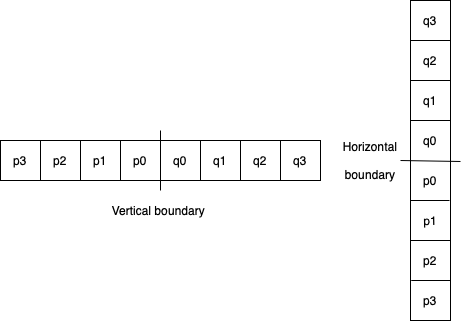
\includegraphics[scale=0.45]{boundary.png}
\caption{Pixels adjacent to vertical and horizontal boundaries}
\label{fig:0}
\end{figure}\\
Secondly, to determine the true boundary for applying deblock filter, two conditions shown as follow should be fulfilled, notice that in our project, thresholds $\alpha$ and $\beta$ are prefixed.
\begin{itemize}
\item |p0 - q0| < $\alpha$
\item |p1 - q1| < $\beta$
\end{itemize}
Thirdly, a 4-tap linear filter is applied with inputs p1, p0, q0, q1 if the filter is applicable. Output value would be assigned to position p0 and q0 as the new value for the filtered boundary. 




%----------------------------------------------------------------------------------------
%	REFERENCE LIST
%----------------------------------------------------------------------------------------
\begin{thebibliography}{50} % Bibliography - this is intentionally simple in this template
%\bibitem{MANUAL}       %\cite{MANUAL}
%Virtual Robot Experimentation Platform USER MANUAL\\
%(www.coppeliarobotics.com/helpFiles/index.html)
\bibitem{PCA}   %\cite{PCA}
Li, Manman.  A Better Color Space Conversion Based on Learned Variances For Image Compression. CVPR Workshops (2019).
\bibitem{deblock}   %\cite{deblock}
H.264/AVC Loop Filter. https://www.vcodex.com/h264avc-loop-filter/. Accessed 02.02.2020.
\end{thebibliography}
\end{document}
